%!TEX root =  main.tex

\documentclass{article}

%% make sure you have the nature.cls and naturemag.bst files where
\usepackage{algorithm}
\usepackage{algorithmic}
\usepackage{amsmath,graphicx}
\usepackage{url}
\bibliographystyle{naturemag}
\usepackage{color}
\newcommand{\comment}[1]{}

\title{Computer vision profiling of neurite outgrowth morphodynamic phenotypes}

%% Notice placement of commas and superscripts and use of &
%% in the author list

%\author{Ludovico Fusco$^{1,7}$, Fethallah Benmansour$^{2, 7}$, Riwal Lefort$^{3, 7}$, Kevin Smith$^{4, 7}$, German Gonzales$^5$,  Catherina Barillari$^6$, Bernd Rinn$^6$, Pascal Fua$^2$, Francois Fleuret$^3$   \& Olivier Pertz$^1$}


%======================================================================
\begin{document}

\maketitle
We developed an image processing pipeline to segments nuclei, somata and neurites and to track them from Time-Lapse High-Content Screens. In the following, we first describe the data and introduce some notations, then we give a detailed description of our processing pipeline. Finally, we describe our evaluation methodology to  assess the quality of the segmentation results.   
%Our approach first detects nuclei and associated somata at each time step. The nucleus of each neuron is detected as a Maximally Stable Extremal Region (MSER)~\cite{Nister:2008} from the Cherry channel. Using the detected nuclei as seed points, a region-growing algorithm segments the neuron�s soma. Next, the implemented multi-objects tracking algorithm~\cite{BerclazTPAMI2011} searches through the full set of nuclei and somata detections to extract the best K-shortest paths according to a similarity measure between two detections. The proposed similarity measure is derived from the Earth Mover�s Distance~\cite{Pele-iccv2009} between the intensity histograms of the detected somata regions (in the supplementary note 3, we show that this distance provides a good tradeoff between efficiency and precision).  Neurons are detected and tracked at an accuracy of (TODO 95\%) (still waiting for the GT to be completed for number crunching); �Finally, the tracked somata are used to initialize a neurite segmentation and association algorithm based on shortest path computation and Voronoi tessellation. Comparison to manually annotated data demonstrates that �(URGENT TODO: crunch the numbers: still waiting for the GT)�
%======================================================
\section{Data description and notations}
%======================================================

We worked with  sequences of two-channel images, one in which the cytoskeleton is marked with Lifeact-GFP. In the other, the nuclei are marked with NLS-mCherry, see the first column of figure \ref{fig:cellBDetection}.

The  input to  our approach  is a  series of  $T$ images  $\mathcal{I}  = \{I_1,
\ldots,  I_t,  \ldots, I_T\}$  from  which  we  extract $K$  nucleus  detections
$d_t^k$.   The  tracking step  described  in Sec.~\ref{sec:tracking}  associates
valid detections  across time steps  while rejecting spurious  detections. Since
each neuron  contains only  one nucleus, there  is a one-to-one  mapping between
each valid  nucleus detection $c_t^i$ and  a neuron $X_t^i$.  Thus, the tracking
task   is   to  provide   a   set   of   neuron  detections   $\mathcal{X}^i   =
\{X_{a}^i,\ldots,X_t^i,\ldots,X_{b}^i \}$ defining an individual neuron $i$ from
time  $t=a$  to $t=b$.   As  depicted  in  Fig.~\ref{fig:notation}, each  neuron
detection $X_t^i$ is composed of a nucleus $c_t^i$, a soma $s_t^i$, and a set of $J$
neurites $N_t^i  = \{n_t^{i,1},  \ldots, n_t^{i,j}, \ldots,  n_t^{i,J} \}$. Thus, a complete neuron
$i$  at time step $t$ is described by $X_t^i = \{ c_t^i, s_t^i, N_t^i \}$.

%----------------------------------------------------------------------------
\begin{figure}[!]
  \begin{center}
       \begin{tabular}{@{\hspace{-1mm}}c}
        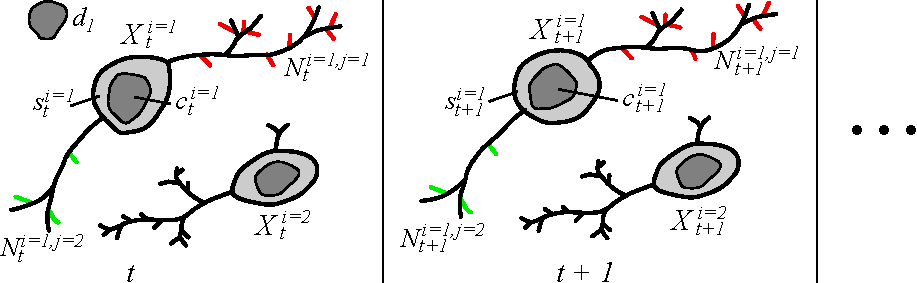
\includegraphics[width = 0.8\linewidth] {images/neurondrawing.pdf}\\ [-2.4ex]
       \end{tabular} 
    \caption{ TODO TODO: no filopodia \footnotesize   Neuron  tracking  notation.  At time $t$ a neuron $i$ detection $X_t^i = \{ c_t^i,
        s_t^i, N_t^i  \}$ contains a nucleus $c_t^i$,  a soma $s_t^i$,
        and    a  set of   neurite-filopodia    tuples    $N_t^i     =    \{(
        n_t^{i,1},F_t^{i,1}),   \ldots,(n_t^{i,j},F_t^{i,j}),  \ldots,
        (n_t^{i,J},F_t^{i,J})  \}$  which  contains $J$  neurites  and
        their associated  filopodia shown in  red for $j=1$  and green
        for  $j=2$. A spurious nucleus  detection  $d_1$ is also shown.
        A neuron $i$  is defined by  a time-series of  neuron detections
        $\mathcal{X}^i     =     \{X_{a}^i,\ldots,X_t^i,\ldots,X_{b}^i
        \}$.  The  tracking returns  a  set  $\mathcal{X}^i$ for  each
        neuron. }
    \label{fig:notation}
  \end{center}
\end{figure}
%% by linking nucleus detections  and ``growing'' the
%%         neuron from the nucleus seed
%----------------------------------------------------------------------------

%======================================================
\section{Neuron segmentation and tracking}\label{sec:neuronSeg}
%======================================================
A three stage neurone segmentation and tracking approach is proposed. First, as described in section \ref{sec:nuc}, we segment nuclei and the associated somata. Since each neuron contains only one nucleus, there is a one-to-one mapping between each valid nucleus and soma,  yielding to a neurone cell body. Second, the cell body tracking step described in section~\ref{sec:tracking}, associates valid cell bodies across time steps while rejecting spurious ones. Finally, using the valid tracked cell bodies, neurites are segmented and tracked over time. 
%----------------------------------------------------------------------------
\subsection{Nuclei and Somata segmentation}\label{sec:nuc}
%----------------------------------------------------------------------------
The  first  step in  our  approach  is to  extract  a  set of  nucleus detections $\{d^1,\ldots,d^K\}$ over the  image series. We worked with two-channel  images where the  cytoskeleton  is marked  with Lifeact-GFP and  nuclei   are   marked   with
NLS-mCherry. The nuclei can be reliably detected as a Maximally Stable Extremal Region (MSER)~\cite{Nister:2008} of the NLS-mCherry channel, and performing a morphological filling operation. The MSER detector finds regions that are stable over a wide range of thresholds of a gray-scale image. For that, we used the \texttt{VLFeat} implementation of MSER\footnote{publicly available at \url{http://www.vlfeat.org/}}. Default parameters of the MSER were used to segment the nuclei except the minimal and maximal size of a nuclei at the given resolution, which were fixed to 70 and 170~~\footnote{Nuclei are considered to have circular shapes with radius varying between 4 and 8 pixels}.  The main advantage of MSER compared to the thresholding approach \cite{Pertzs11} is its robustness and insensitivity to contrast change.  


Using the nuclei as seed regions, somata are segmented using a region growing and region competition algorithm on the Lifeact-GFP channel, called the \textit{green} channel.
This is done by launching a propagating front from all the detected nuclei simultaneously. 
For a given image frame, let $\{d^1, \cdots, d^K \}$ be the set of detected nuclei.
To segment the somata, we first compute a solution of the Eikonal equation 
\begin{equation}\label{eq:eikonal}
\|\nabla \mathcal{U} \| = \mathcal{P} \text{~~~~such that~~~~} \mathcal{U}(d^k) = 0,
\end{equation}
where $\nabla \mathcal{U}$ is the gradient of a distance $\mathcal{U}$ to be computed and
\begin{equation}\label{eq:potential}
\mathcal{P}(x) = \frac{1}{A \exp\left(- \frac{(I(x) - \mu_k)^2}{2 \beta^2 \sigma_k^2}\right) + 1},
\end{equation}
$k$ being the index of the closest nuclei detection $d_k$ to the pixel location $x$, and $I(x)$ being the associated green intensity, $\mu_k$ and $\sigma_k$ being respectively the mean and standard deviation of the green intensities of the pixels describing $d_k$. Parameter $\beta$, is a multiplicative factor of the intensity standard deviation $\sigma_k$, and represents a tolerance of variation between the local foreground (somata) intensities and the local background intensities.

$\mathcal{U}$ defines a geodesic distance to the detections $d^k$. It combines the local intensity differences and the euclidean distance. From equation \ref{eq:potential}, one can see that the more the green intensity of a pixel $I(x)$ is different from the mean intensity of the closest detected nuclei $\mu_k$, the higher the potential $\mathcal{P}$ would be, and from equation \ref{eq:eikonal}, the higher $\mathcal{U}$ would be. The algorithm to compute the geodesic distance $\mathcal{U}$, is a variant of the Fast Marching algorithm \cite{Cohen96,Sethian99} introduced in \cite{BenmansourC09}.

The somata segmentations are finally obtained by thresholding both $\mathcal{U}$ and the euclidean distance to the nuclei (those 2 shresholds are denoted $\mathcal{T}_g$ and $\mathcal{T}_e$ repectivelly). An example for nuclei and somata segmentation is depicted on figure \ref{fig:cellBDetection}. For all our experiments, we took $A = 1e7$, $\beta = 1.5$, $\mathcal{T}_g = 2e-6$ and $\mathcal{T}_e = 7$.

%----------------------------------------------------------------------------
\begin{figure}[!b]
  \begin{center}
       \begin{tabular}{@{\hspace{1mm}}c@{\hspace{1mm}}c}
        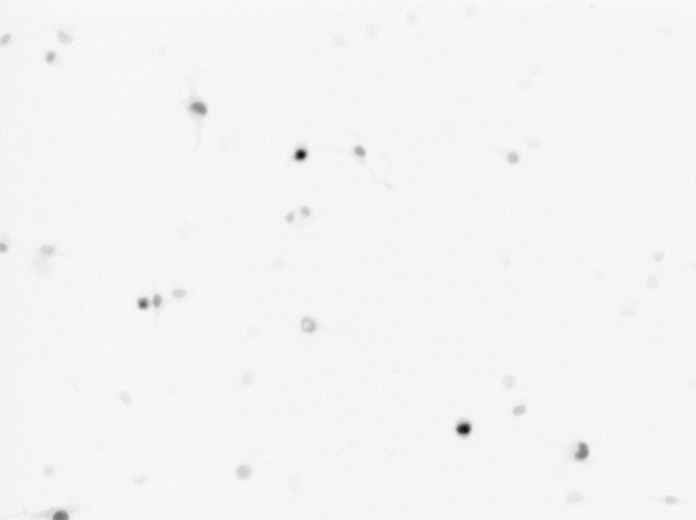
\includegraphics[width = 0.49\textwidth] {images/OriginalRed.png} & 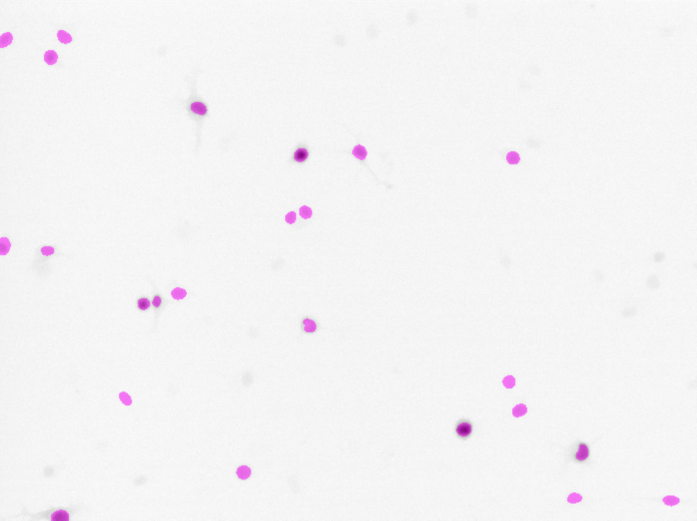
\includegraphics[width = 0.49\textwidth] {images/NucleiDetectionRed.png}\\ 
	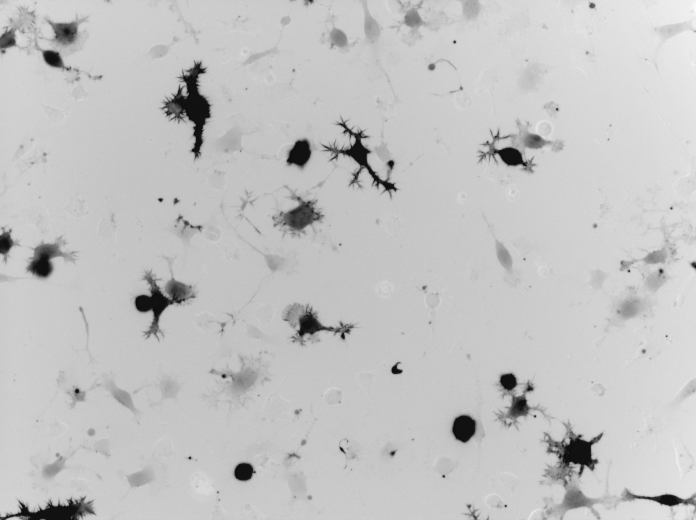
\includegraphics[width = 0.49\textwidth] {images/OriginalGreen.png} & 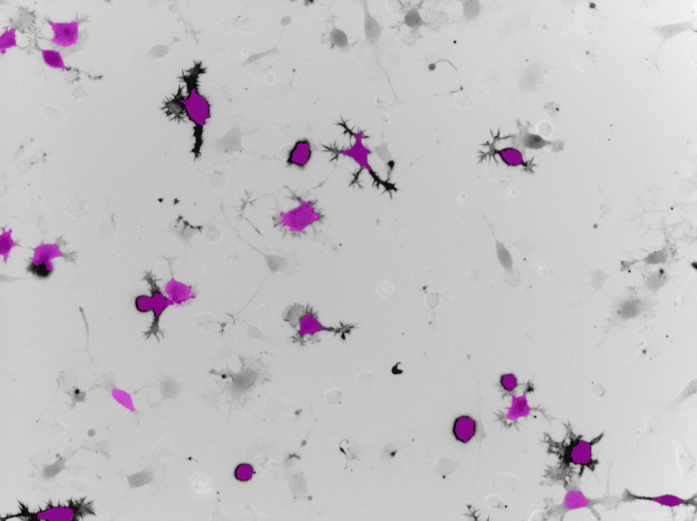
\includegraphics[width = 0.49\textwidth] {images/SomataDetectionGreen.png}\\ 
       \end{tabular} 
    \caption{ \footnotesize  Cell body detection. On the first row, nuclei detections overlaid on top of the NLS-mCherry channel. On the second row, somata detections overlaid on top of the Lifeact-GFP channel. From left to right: the original image, and the automatic detections.}
    \label{fig:cellBDetection}
  \end{center}
\end{figure}
%----------------------------------------------------------------------------

At this point, cell body detections $d_t^i = (c_t^i, s_t^i)$ have been obtained form the whole sequence. A filtering step is applied to these detections to keep only the most reliable ones. First, detections that are too close to the image boundary (with distance less than 10 pixels) are ignored. Second, the minimal tolerated circularity is 0.2. Finally, the maximal accepted eccentricity is 0.85. 


%----------------------------------------------------------------------------
\subsection{Cell body tracking}\label{sec:tracking}
%----------------------------------------------------------------------------

The tracking algorithm searches through the full set of nuclei detections
and iteratively associates the most similar  pairs of detections, returning
lists of valid detections corresponding to each neuron $\mathcal{X}^i$.
This is accomplished by constructing a graph 
$\mathcal{G}=(\mathcal{D},\mathcal{E})$  where each
node $d^k_t  \in \mathcal{D}$  corresponds to  a detection. 
For each detection $d^k_t$ in time step $t$, edges $e \in \mathcal{E}$ are formed between
$d^k_t$ and all past and future detections within a time window $W$.
A weight $w_e$ is assigned to each edge according to spatial and 
temporal distances, and a shape measure 
$w_{e} = \alpha || d^k_{t1} - d^l_{t2} ||
+ \beta |t1 - t2| + \gamma f(\nu^k_{t1}, \nu^l_{t2})$
where $e^{k,l}$ connects  $d^k_t$ and $d^l_t$, and $\nu^k$  is a shape
feature vector  containing $d^k_t$'s area,  perimeter, mean intensity,
and major  and minor axis lengths  of a fitted  ellipse. $f$ evaluates
differences between  a feature $a$ extracted from  $d^k_t$ and $d^l_t$
as  $f(a^k,a^l) =  \frac{|a^k  - a^l|}{|a^k  +  a^l|}$.  The  tracking
solution  corresponds   to  a  set  of   edges  $\mathcal{E'}  \subset
\mathcal{E}$ that minimizes the cost $\sum_{e \in \mathcal{E'}} w_e$.

%( f(a^k,a^l) + f(ma^k,ma^l) + f(mn^k,mn^l) + f(ec^k,ec^l) + f(p^k,p^l) + 
%f(\hat{I}(d^k), \hat{I}(d^l) )$

%detections found in past $t-W \ldots t-1$ and future
%$t+1 \ldots t$ time steps.

%Edges $\mathcal{E}$ fully connect detections between time steps

%%  Graph edges
%% $\mathcal{E}$ are created between  detections belonging to a different
%% time frame  in a given  time window $W$.  A cost $c_e$ is  assigned to
%% each  edge  $e \in  \mathcal{E}$  according  to  spatial and  temporal
%% distances and  shape proximity. The  tracking output corresponds  to a
%% set  of edges  $\mathcal{E'} \subset  \mathcal{E}$ that  minimizes the
%% cost $\sum_{e \in \mathcal{E'}} c_e$.

To minimize this cost function,  we adopt a greedy selection algorithm
outlined     in    Table~\ref{algo:greedy}    and     summarized    in
Fig.~\ref{fig:greedytracking}  that iteratively  selects an  edge with
minimum  cost  $\hat w_e$  and  adds  it  to the  set  $\mathcal{E}'$,
removing  future   and  past   connections  from  the   detections  $e^{k,l}$
connects. The algorithm iterates until  the minimum cost $\hat w_e$ is
greater than  a threshold $T$. The  track for neuron  $i$ is extracted
from       $\mathcal{E}'$      by      traversing       the      graph
$(\mathcal{G},\mathcal{E}')$  and appending linked  nucleus detections
to $\mathcal{X}^i$.

%-----------------------------------------------------------------
\begin{algorithm}[h!]
\caption{Greedy tracking association algorithm}
\begin{algorithmic}[100]
%\STATE A graph $\mathcal{G}=(\mathcal{V},\mathcal{E})$ is created where each node $v \in \mathcal{V}$ is associated to a detection.
%\STATE Graph edges $(u,v) \in \mathcal{E}$ are created between detections belonging to a different time frame in a given time window $W$.
%\STATE A weight $c_e$ is assigned to each edge according to spatial and temporal distance and shape.
\STATE Start with an empty set $\mathcal{E}'$.
\REPEAT
\STATE Find edge $\hat e^{k,l}$ with minimum cost $\hat w_e$.
\STATE Add $\hat e^{k,l}$ to $\mathcal{E}'$, linking detections $d^k_{t1}$ and $d^l_{t2}$.
\STATE Remove $\hat e^{k,l}$ from $\mathcal{E}$.
\IF {$ t1 < t2 $}
\STATE Remove edges between $d^k_{t1}$ and {\em future} detections (where $t > t1$) from $\mathcal{E}$
\STATE Remove edges between $d^l_{t2}$ and {\em past} detections (where $t < t2$) from $\mathcal{E}$
\ELSE
\STATE Remove edges between $d^k_{t1}$ and {\em past} detections (where $t < t1$) from $\mathcal{E}$
\STATE Remove edges between $d^l_{t2}$ and {\em future} detections (where $t > t2$) from $\mathcal{E}$
\ENDIF
\UNTIL{$\hat w_e > T$}
\end{algorithmic}
\label{algo:greedy}
\end{algorithm}
%-----------------------------------------------------------------


%----------------------------------------------------------------------------
\begin{figure}[t]
  \centering
       \begin{tabular}{c}
        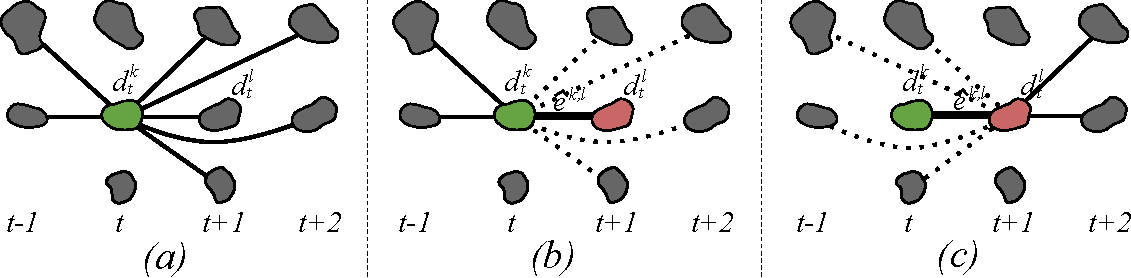
\includegraphics[width = 100mm] {images/greedytracking.pdf}\\ [-2.4ex]
       \end{tabular} 
    \caption{  {\footnotesize {\it Greedy  Tracking.}  {\em  (a)} The algorithm begins with each
        detection fully connected to all future and past detections
        within  a time  window  $W$.  Above, only  $d^k_t$'s edges  are
        shown. {\em  (b)} Each iteration,  the edge $\hat{e}^{k,l}$
        with   minimum  cost   $\hat{w}_e$  is  added  to $\mathcal{E}'$.   Edges  connecting
        $d^k_t$ to  future detections are  removed from $\mathcal{E}$.
        {\em  (c)} Edges  connecting  $d^l_t$ to  the past  are
        removed from $\mathcal{E}$.  The process is repeated until $\hat w_e > T$. }}
    \label{fig:greedytracking}
  
\end{figure}

The parameters of this algorithm have been fixed empirically as follows: $W = 4$, $\alpha = 1$, $\beta = 50$, $\gamma = 40$ and $T = 200$. Only tracks containing at east 20 frames are kept. In addition to these parameters, a spatial connection constraint is applied during the construction of the graph $\mathcal{G}$. In fact, only detections that are at distance less than 50 pixels are connected to create the set of edges $\mathcal{E}$.

Once the tracking is achieved, tracks are sorted according to their total cumulated green intensities, and only the 20 best tracks are kept.

%----------------------------------------------------------------------------
\subsection{Neurites segmentation and association}\label{sec:neurites}
%----------------------------------------------------------------------------
\label{sec:segmentation}
\vspace{-2mm}
Given an  image $I_t$  and the set  of somata  present in it  $S_t=\{s_t^1 \dots
s_t^m \}$,  our goal is  to associate  to each pixel  $u$ a label  $J_t(u)$ that
indicates to which soma it belongs.   The probability of $J_t(u)$ can be deduced
using Bayes' rule,
%\vspace{-1mm}
\begin{equation}
  \label{eq:bayes}
  P(J_t(u)=i|S_t,I_t) = \frac{P(S_t,I_t| J_t(u)=i)}{\sum_{\eta=1}^m P(S_t,I_t|J_t(u)=\eta)},
\end{equation}
\noindent  where we  have assumed  a uniform  distribution on  $P(J_t(u))$.  The
numerator  is modeled  as the  probability of the path $L$ that connects maximally 
the voxel $u$ to the soma $s_t^i$,
%% \begin{equation}
%%   \label{eq:shortestpath}
$  P(S_t,I_t| J_t(u)=i) = \max_{L:u\rightarrow  s_t^i}   \prod_{\{l_{r}\}
    \in L  } P(I_t(r)|l_{r}),$
%\end{equation}
where $l_{r}$ are indicator  variables for the locations forming the
path $L$. We chose this model  since an optimal maxima can be found
by minimizing its  negative likelihood using geodesic shortest  path \cite{Cohen96} and because
it produces connected components.

The extraction of neurites from a time frame $I_t$ proceeds in the following stages:
\begin{itemize}
\item Compute tubularity measure $T_t$ as in \cite{Frangi98}. In addition, detected but not tracked somata are ignored.
\item Estimate the parameters of a sigmoid functions which is applied to the tubularity measure to obtain a potential $P_t$ that drives the Fast Marching algorithm \cite{Cohen96,Sethian99}.
\item Launch simultaneously the front propagation Fast Marching algorithm from all the tracked somata. This is done by solving the Eikonal equation $\|\nabla \mathcal{U}_t \| = P_t$. That yields a geodesic distance map $\mathcal{U}_t$ and the associated tessellation $\mathcal{V}_t$. The complexity of the algorithm, at this stage, does not depend on the number of tracked somata but depends only on the size of the image. 
\item Threshold the geodesic distance with a soft threshold $\mathcal{T}_s$, and then extract local maxima of $\mathcal{U}_t$ in each thresholded region\footnote{the local maxima are obtained using the Matlab function \texttt{imregionalmax}}
\item Using the Geodesic distance $\mathcal{U}_t$, back-propagate from all the local maxima, by keeping only points for which the value is above a hard threshold $\mathcal{T}_h$
\item Finally, we instantiate a Minimum Spanning Tree from each root touching a soma, and create the associated neurite tree.
\end{itemize}

The different steps of our approach are illustrated in figure \ref{fig:NeuritesDetection}.



%To optimize this function, we first compute geodesic distances from the tracked somata using the fast marching algorithm \cite{Sethian99,Cohen96}, applied on $P(I_t(v)|v)$, where $P(I_t(v)|v)$ represents the probability that a  neurite traverses a node $v$ and is
%obtained  by  applying  a  sigmoid  function  to  the  output  of  the
%tubularity filter  of~\cite{Frangi98}.  The parameters  of the sigmoid
%function are  estimated using  maximum likelihood. 
%
%Finally,  we define the set  of neurite pixels $U_n^t$  as those that connect  to any soma
%with a higher probability than $\epsilon$.  We predict their labels as
%the  ones  that  maximize   Eq.~\ref{eq:bayes}.   The  set  of  pixels
%associated to neuron $X_t^i$ is the union of the neurites and the soma
%associated  with $i$, $  U_i^t =  \{u \in  U_n^t |  J_t(u) =  i\} \cup
%s_t^i$. To reduce  the neurite segmentation to a  tree, we skeletonize
%the neuron and  define as root node the pixel  of the skeleton closest
%to the centroid of the nucleus. We instantiate a Minimum Spanning Tree
%from the  root and create a  neurite tree every time the  the spanning tree
%exits the soma.
%

%----------------------------------------------------------------------------
\begin{figure}[!h]
  \begin{center}
       \begin{tabular}{@{\hspace{1mm}}c@{\hspace{1mm}}c@{\hspace{1mm}}c@{\hspace{1mm}}c}
        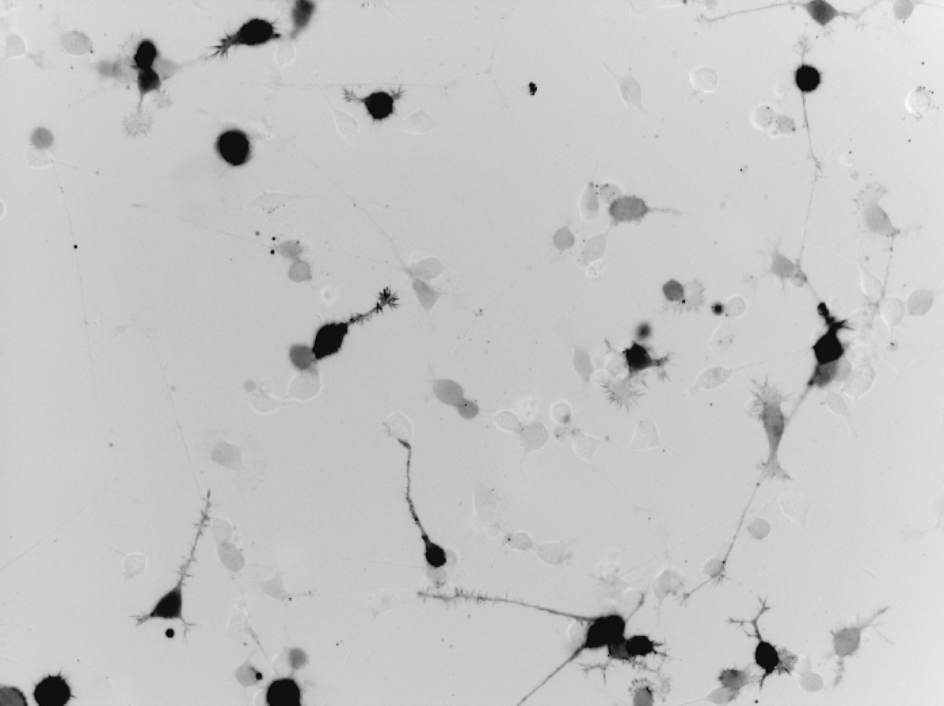
\includegraphics[width = 0.24\textwidth] {images/Figures_172_50/Original.png} & 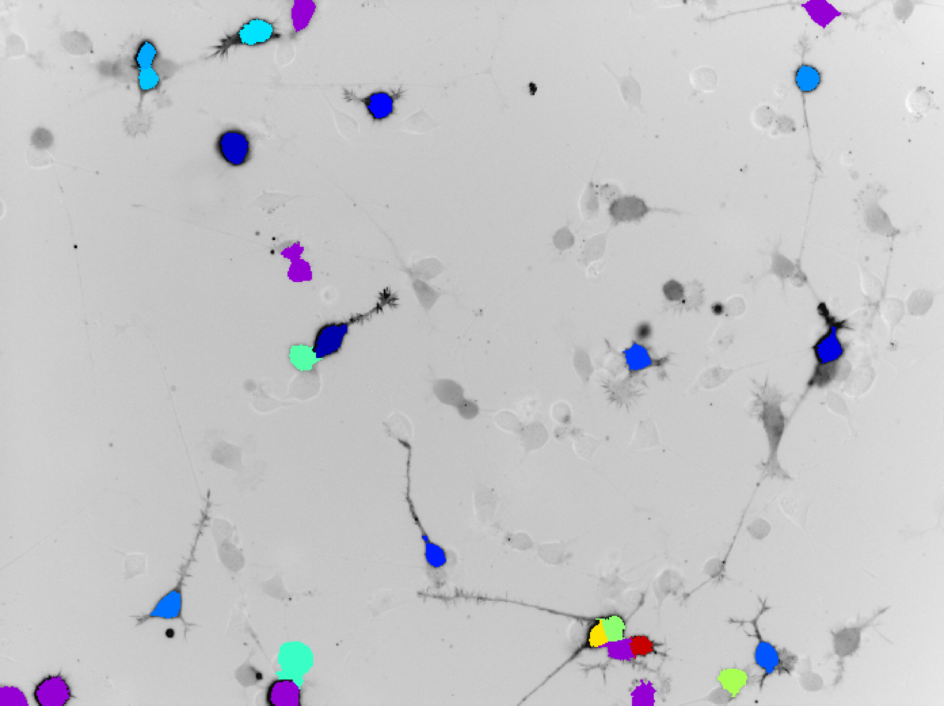
\includegraphics[width = 0.24\textwidth] {images/Figures_172_50/DetectedSomata.png} & 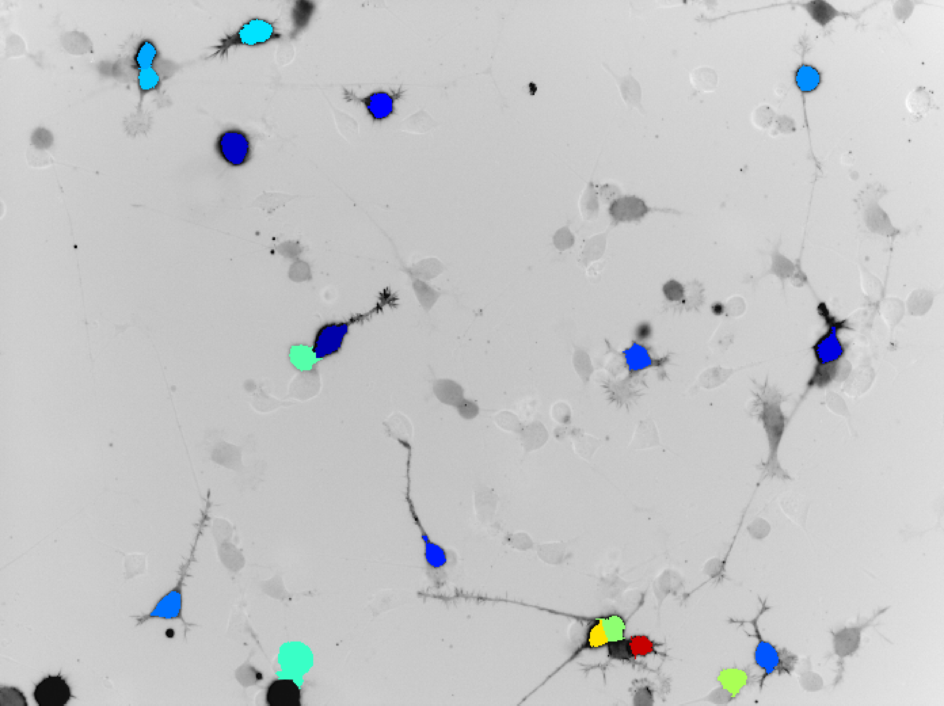
\includegraphics[width = 0.24\textwidth] {images/Figures_172_50/TrackedSomata.png} & 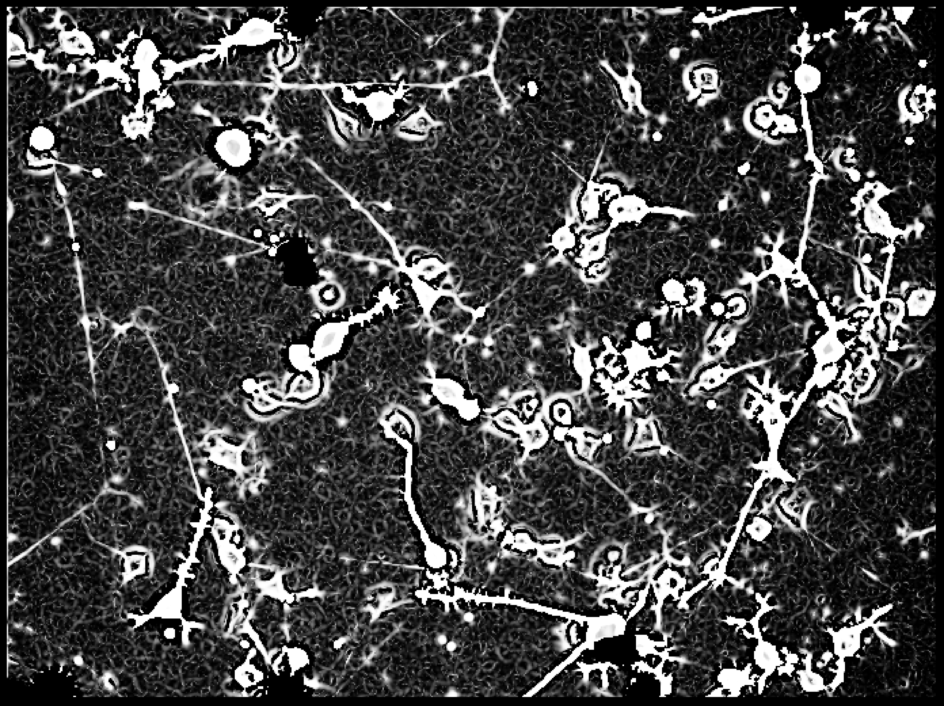
\includegraphics[width = 0.24\textwidth] {images/Figures_172_50/Frangi.png}\\
        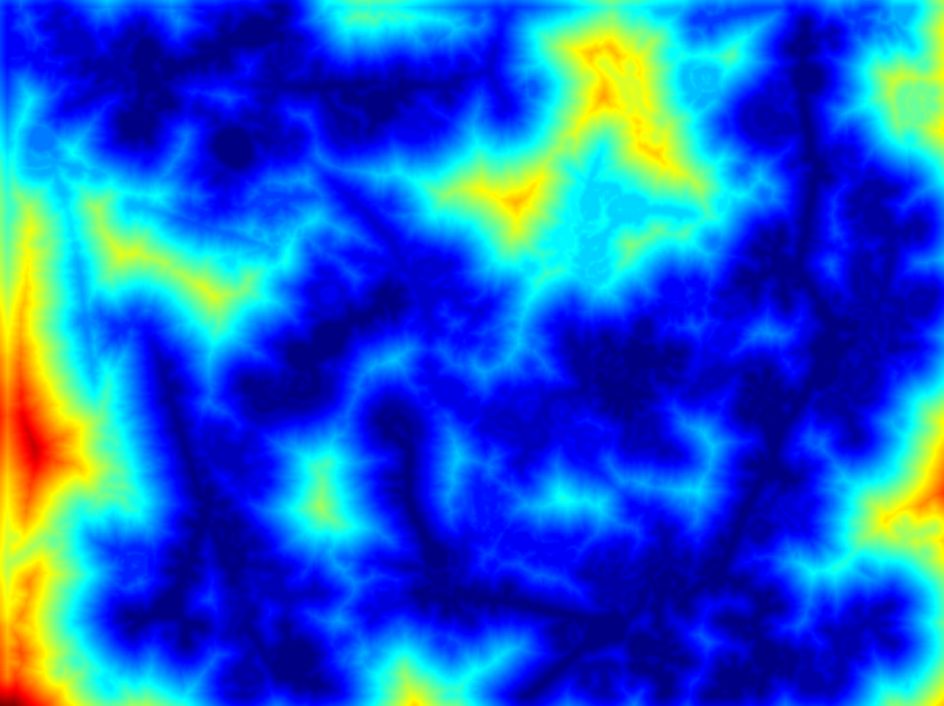
\includegraphics[width = 0.24\textwidth] {images/Figures_172_50/GeodesicDistance.png} & 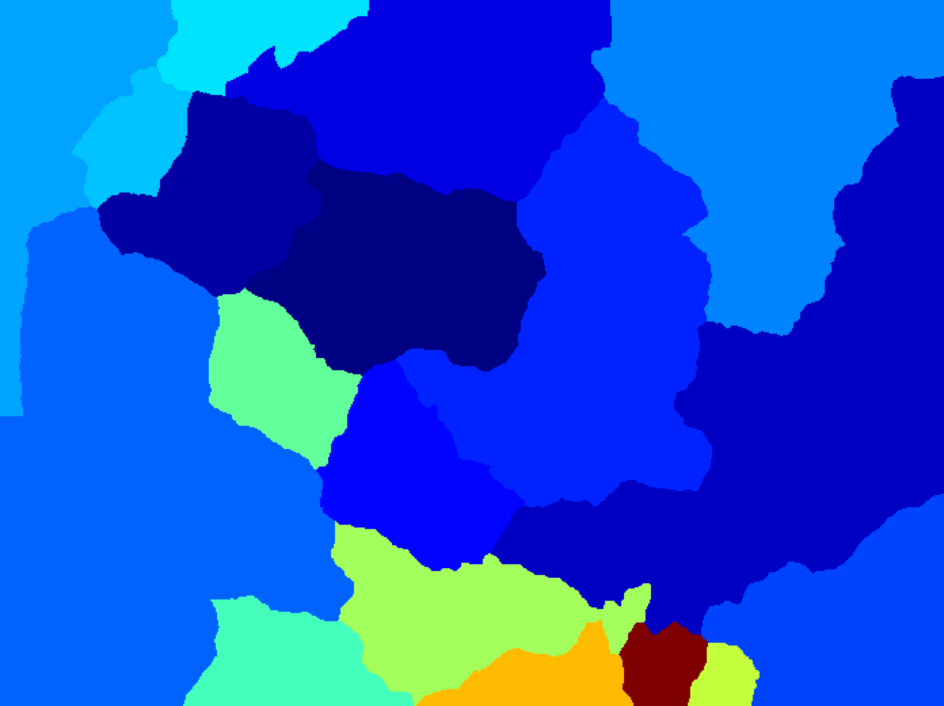
\includegraphics[width = 0.24\textwidth] {images/Figures_172_50/GeodesicRegions.png} & 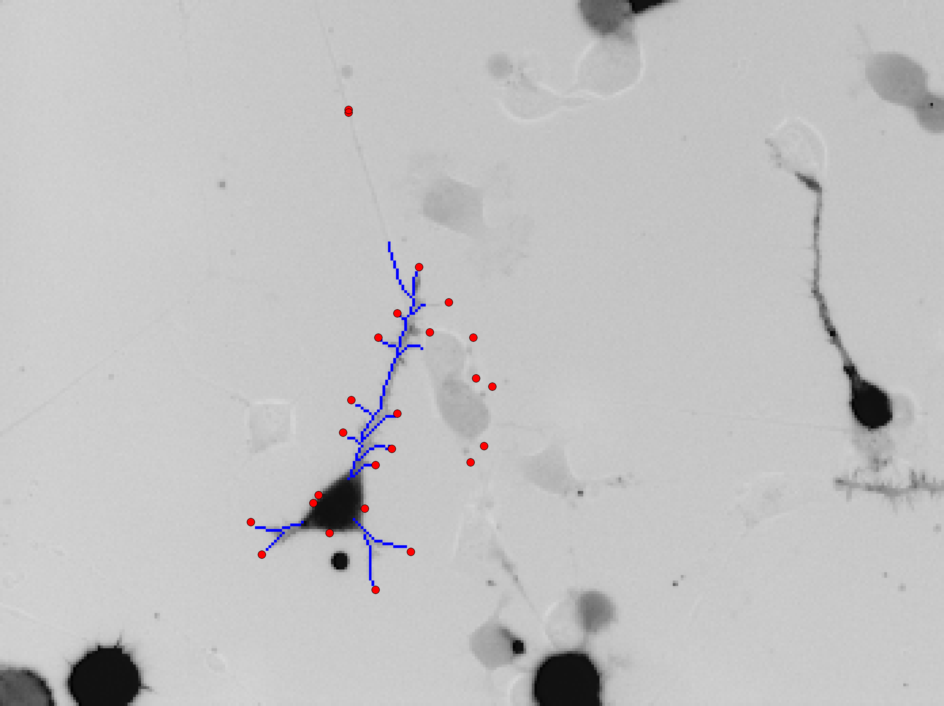
\includegraphics[width = 0.24\textwidth] {images/Figures_172_50/DetectedNeurites8.png} & 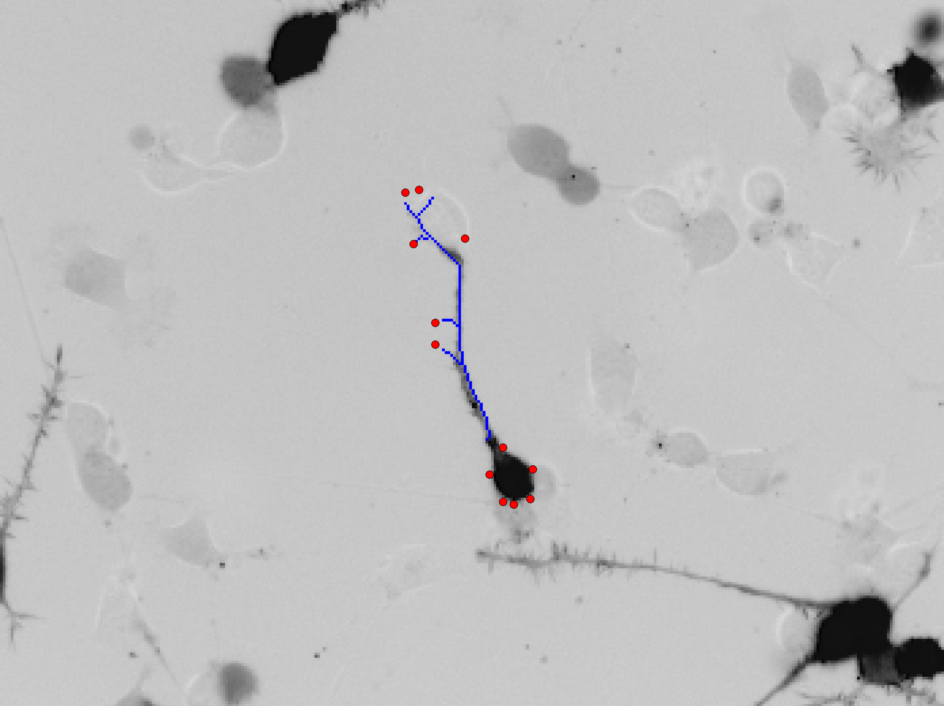
\includegraphics[width = 0.24\textwidth] {images/Figures_172_50/DetectedNeurites5.png} 
       \end{tabular} 
    \caption{ \footnotesize  Neurites detection. From left to right, top to bottom : -Original image (only the green channel is displayed). -Both tracked and detected somata are overlaid on top of the original image. Detected but not tracked somata are coloured with dark violet. -Only tracked somata are overlaid on top of the original image. - Potential $P_t$, based on the tubularity measure of \cite{Frangi98}. -Geodesic distance $\mathcal{U}_t$ computed from the tracked somata. Blue corresponds to low values and red to high values. - The Voronoi tessellation $\mathcal{V}_t$ associated to the geodesic distance. Each colour represent a region. -The last two figures are closeup looks of the original image illustrating the last steps of our neurite detection algorithm: first, local maxima of the soft thresholded regions are displayed in red, then the hard thresholded back propagation pixels are shown in blue.}
    \label{fig:NeuritesDetection}
  \end{center}
\end{figure}
%----------------------------------------------------------------------------

Parameters of the neurite detection algorithm are as follows:
\begin{itemize}
\item Frangi \cite{Frangi98} parameters are: \texttt{ FrangiOpt.FrangiScaleRange = [1 2], FrangiOpt.FrangiScaleRatio = 1, FrangiOpt.FrangiBetaOne = .5, FrangiOpt.FrangiBetaTwo = 15,}, 
\item Geodesic distance thresholds: $\mathcal{T}_s = -\log(10^{-4})$, and $\mathcal{T}_h = -\log(0.2)$.
\item Finally, any neurite containing less than 10 pixels have been ignored.
\end{itemize} 


%\subsection{Evaluation}
%
%
%A detection, either a nucleus or a somata, is considered positive if there exist a ground truth object (of the same kind) overlapping sufficiently with it.  More formally, a detection $d$ is considered as a positive detection if there exist a ground truth object $g$ such that $\displaystyle \frac{g\cap d}{g\cup d} > 80\%$.
%
%\begin{itemize}
%\item On the 10x dataset, and over the 3 annotated sequences, only 28 nuclei have not been detected. That represents {\bf{1.3\%}} of miss detections.
%\item On the 20x dataset,  and over the 12 annotated sequences, 101 nuclei have not been detected. That represents {\bf{2.14\%}} of miss detections.
%\end{itemize}
%
%Since the ground truth is not complete, in other words, some visible cells have not been annotated, then we do not count the false positive detections. 




%======================================================
\subsection{Neurite Tracking}\label{sec:neuriteTracking}
%======================================================

Neurites are tracked by applying the algorithm described in Sec~\ref{sec:tracking} using
the centroids of the neurite trees instead of nucleus centroids, with the additional 
constraint that edges may only exist between neurites that emanate from the same tracked soma and only from consecutive time detections. The weight $w_e$ of an edge connecting two neurites $N^i_t$ and $N^j_{t'}$is assigned according to spatial distance and a shape measure $w_e = w_{TCL}f(\text{TotalCableLenght}(N^i_t), \text{TotalCableLenght}(N^j_{t'})) + w_{\text{Centroid}} \|\text{Centroid}(N^i_{t}) - \text{Centroid}(N^j_{t'})\| + w_{\text{SomaContact}} \|\text{SomaContact}(N^i_{t}) - \text{SomaContact}(N^j_{t'})\|$, where $w_{TCL} = 50$, $w_{\text{Centroid}}  = 10$, $w_{\text{SomaContact}}  = 5$, $\text{TotalCableLength}(N)$ is the total cable length of a neurite $N$, $\text{Cenrtoid}(N)$ is its centroid, $\text{SomaContact}(N)$ is its contact point with the soma, and $f(a^k,a^l) =  \frac{|a^k  - a^l|}{|a^k  +  a^l|}$. As opposed  to the weights used for cell body tracking, the weights used here for neurites tracking do not include a temporal distance because the neurites are associated to already tracked cell bodies.

During the neurite tracking stage, only neurites that are considered stable have been taken into account.
Neurites are considered stable if their total cable length is above 30 pixels. The threshold parameter of the tracking algorithm (Algorithm 1), have been adapted to neurites by taking $T = 800$.

%======================================================
\section{Evaluation}
%======================================================

The image processing pipeline, described in section \ref{sec:neuronSeg}, segments and tracks cell bodies and neurites.
Questions one could raise to evaluate the quality of the segmentation results are:
\begin{enumerate}
\item What is the quality of the cell body components segmentation. More precisely, what is the quality of the nuclei and the somata segmentations. (Static evaluation)
\item What is the quality of the cell body tracking (cell identity assignment). In other words, does the algorithm track accurately the moving cells? and is it able not to switch identities of two neighbouring moving cells? (Dynamic evaluation)
\item Are the neurites segmented accurately? Neurite trees are complex structures, and are critical to our phenotypic study. How can we asses their quality is a crucial question to answer (Static evaluation)
\item Are the neurites tracked properly? or a simpler question could be : how accurate is the "neurite to cell body" assignment step? (Dynamic/Static evaluation ?)
\end{enumerate}

In order to evaluate our algorithm in a fair manner, one should bear in mind that, at detection time, we made the choice not to detect and track all visible cells and neurites. For instance, a neurone that enters the field of view for a short period of time (say during 5 frames, for instance) is not kept in the final set of tracks. In addition, as described in section \ref{sec:tracking}, tracked cells are sorted according to their cumulated green intensity, and only the 20 best tracks are kept. We made this choice to favours cell body tracks that are bright with a long lifetime. This choice is also justified by the fact that the moving neurons appears with very different contrast: some are very bright and others are quite faint. Assuming that the algorithm will be able to segment and track accurately all the moving neurons is not realistic, and we preferred to focus our efforts in segmenting and tracking accurately the most robust neurons. 

In order to evaluate the different critical components of our processing pipeline we need to annotate \textit{ground truth} data. If one annotates all visible moving neurones, then our segmentation results will be penalised by the objects that have been purposefully ignored by the algorithm. Hence, evaluation scores obtained using such an over complete ground truth would not reflect the quality of the segmentation and tracking results. To sumup, a special care must be made for the ground truth annotation step and for the quantitative evaluation. 

In the next sections, we will describe the ground truth annotation protocol and the evaluation methodology for each of the critical  steps of our processing pipeline.

%======================================================
\subsection{Evaluating Cell body detection }
%======================================================
To manually segment nuclei and somata from dynamic sequences, we used \texttt{TrakEM2}\footnote{publicly available at \url{http://www.ini.uzh.ch/~acardona/trakem2.html}}, a plugin of \texttt{FIJI/ImageJ}\footnote{\url{http://fiji.sc/Fiji}}. To ease the annotation step, the input sequences have been encoded in a single multipage tiff file for each channel, and an xml file have been generated for each sequence to encode the segmentation and tracking data structure.

A set of instructions was given to 3 different experts to annotate the data:
\begin{itemize}
\item segment and track only cell bodies that are bright and that have a long enough lifetime
\item segment carefully the nuclei and the somata
\item keep track of the identities of the segmented cell bodies
\end{itemize}

Three sequences have been randomly selected from our dataset dataset. From these sequences, 29 cells have been tracked, representing 2152 annotated nuclei and somata.


A detected object, either a nucleus or a soma, is considered positive if there exist a ground truth object (of the same kind) overlapping sufficiently with it.  More formally, a detection $d$ is considered as a positive detection if there exist a ground truth object $g$ such that $\displaystyle \frac{g\cap d}{g\cup d} > 80\%$.


On our ground truth dataset, and over the 3 annotated sequences, only 28 nuclei have not been detected,  representing {\bf{1.3\%}} of miss detections.
%\begin{itemize}
%\item On the 10x dataset, and over the 3 annotated sequences, only 28 nuclei have not been detected. That represents {\bf{1.3\%}} of miss detections.
%\item On the 20x dataset,  and over the 12 annotated sequences, 101 nuclei have not been detected. That represents {\bf{2.14\%}} of miss detections.
%\end{itemize}

%\begin{itemize}
%\item 12 sequences have been randomly selected from the \texttt{20x} dataset. From these sequences, 79 cells have been tracked, representing 4709 annotated nuclei and somata.
%\item 3 sequences have been randomly selected from the \texttt{10x} dataset. From these sequences, 29 cells have been tracked, representing 2152 annotated nuclei and somata.
%\end{itemize}
%%----------------------------------------------------------------------------
%\subsection{Ground truth}
%%----------------------------------------------------------------------------
%In order to evaluate our automatic algorithm, we manually annotated cell bodies and neurites using appropriate tools as described hereinafter.
%We clearly distinguished between two annotation tasks: 
%\begin{itemize}
%\item segmentation and tracking of nuclei and somata from dynamic sequences,
%\item segmentation of neurite trees from static images.
%\end{itemize}
%We clearly made this distinction because we could not find an appropriate semi-automatic or manual software for tracking the neurites. Therefore, even if our automatic pipeline is able to track neurites, only the quality of neurite trees at a given time frame will we assessed.
%
%Our computer vision pipeline have been applied to two different sets of sequences acquired using two different magnifications: \texttt{10x} and \texttt{20x}. Therefore, we made random selections from each magnification set, and conducted our evaluation on each of them independently.
% 
%\subsubsection{Cell body ground truth}


%
%\subsubsection{Neurite ground truth}
%To segment neurite trees from static images, we used an improved version of the Simple Neurite Tracer (SNT) plugin. The SNT plugin\footnote{\url{http://fiji.sc/wiki/index.php/Simple_Neurite_Tracer}}, a FIJI plugin, is a semi-automatic tool meant to reduce user' interaction for neuronal tree tracing . Recently, an improved version of SNT have been released \url{http://cvlab.epfl.ch/software/delin/index.php}, allowing a better description of the neurite branches, including their width estimate and more accurate centeline extraction as shown in figure~\ref{fig:annotations}.
%
%Similarly to the dynamic dataset, we randomly selected images from the two different magnification sets, and annotated all visible neurite trees:
%\begin{itemize}
%\item 30 images from the 20x dataset have been randomly selected. 223 neurite trees or neurite branches have been annotated.
%\item 27 images from the 10x dataset have been randomly selected. 257 neurite trees or neurite branches have been annotated.
%\end{itemize}
%
%Filopodia have been annotated only on images from the 20x dataset.
%%----------------------------------------------------------------------------
%\begin{figure}[!t]
%  \begin{center}
%       \begin{tabular}{@{\hspace{1mm}}c@{\hspace{1mm}}c}
%        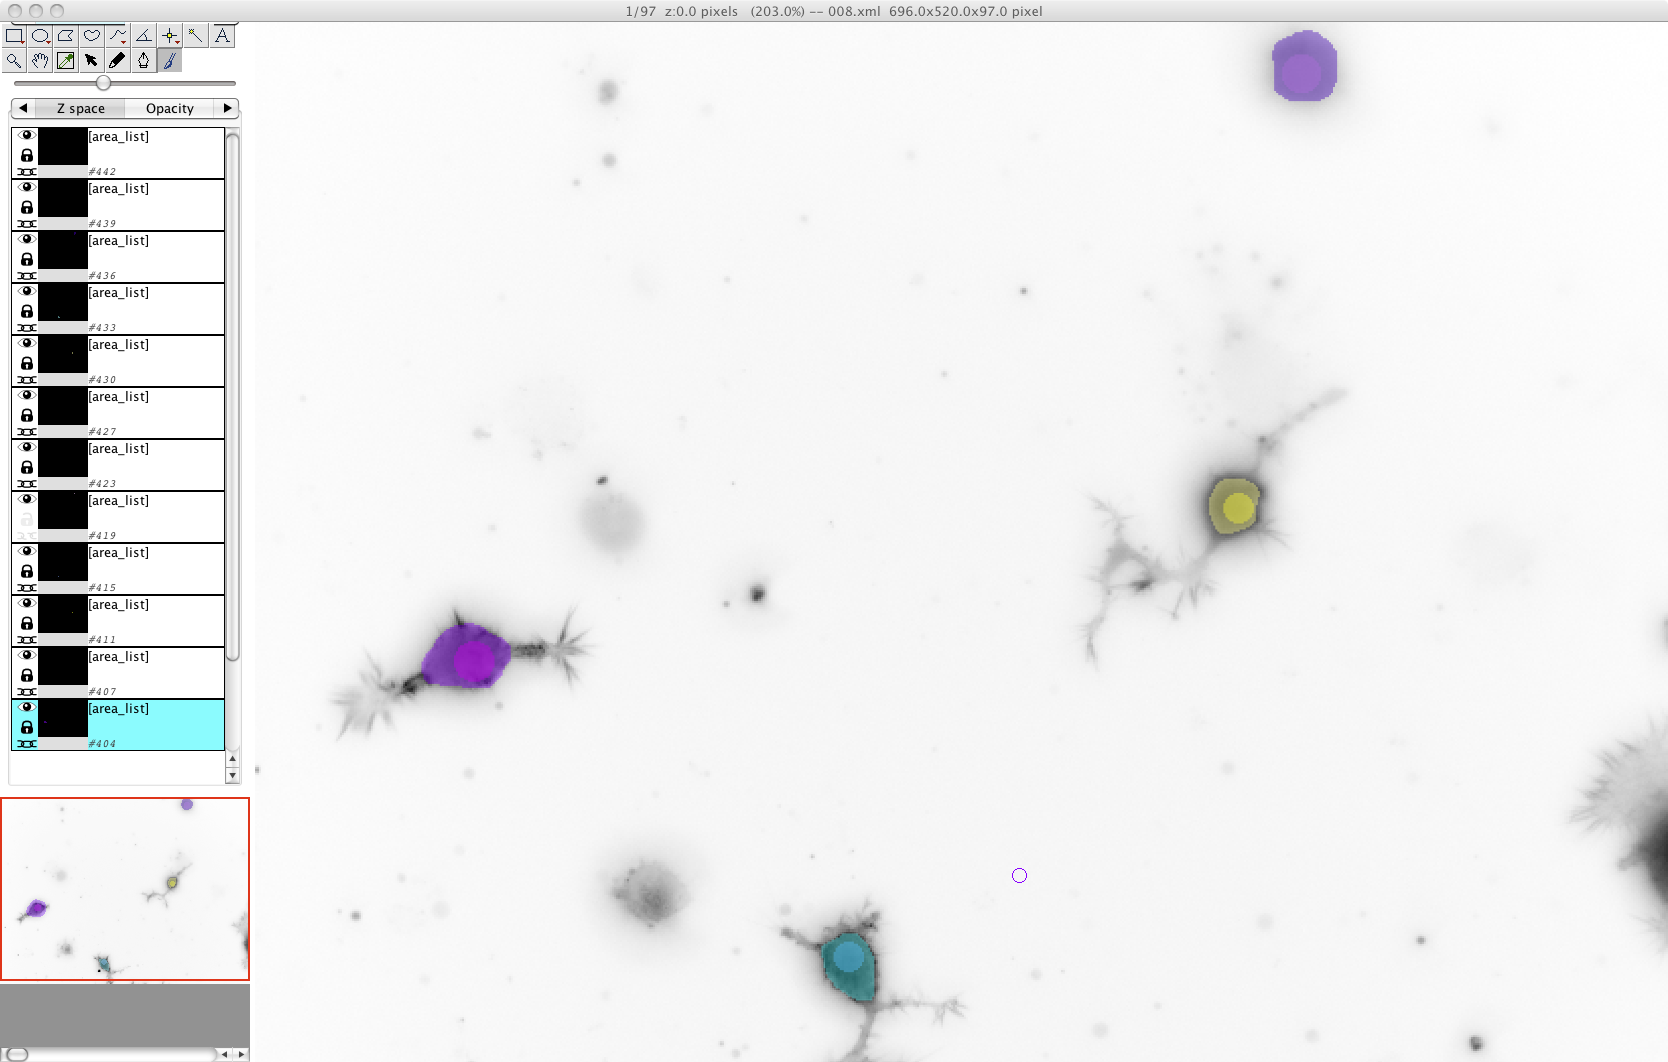
\includegraphics[width = 0.5\textwidth] {images/TrakEM2_Example.png} & 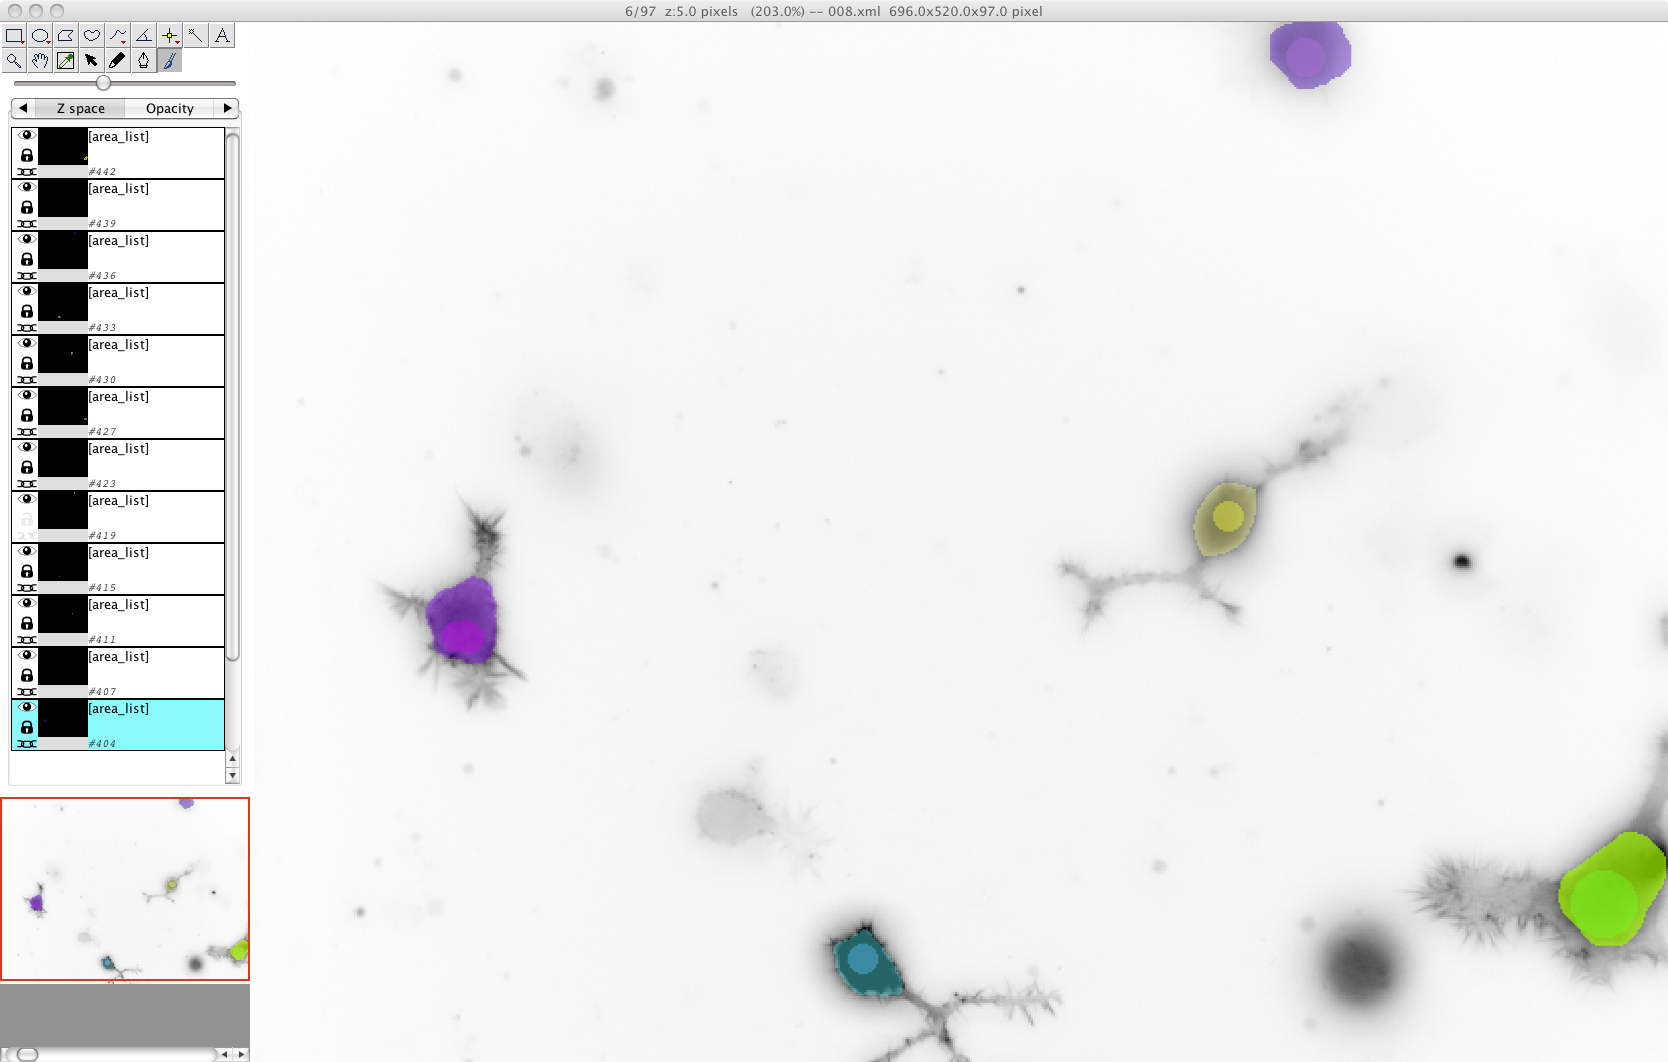
\includegraphics[width = 0.5\textwidth] {images/TrakEM2_Example2.png}\\
%                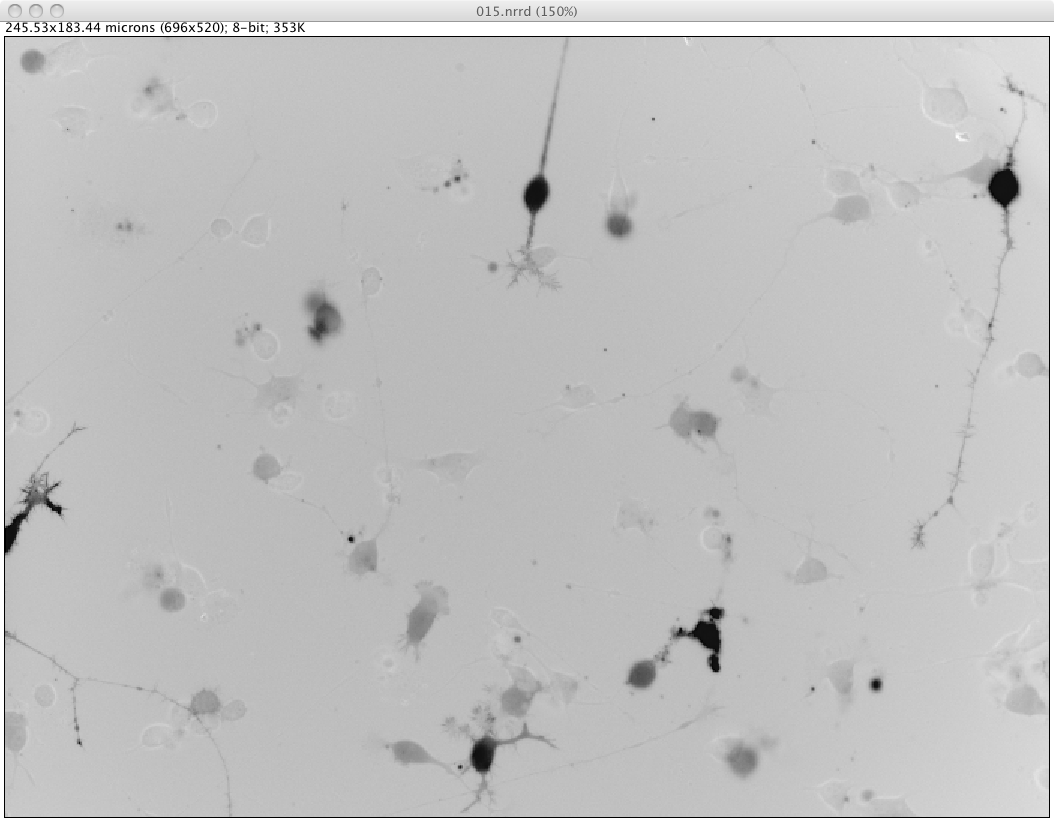
\includegraphics[width = 0.5\textwidth] {images/SNT_015_Or.png} & 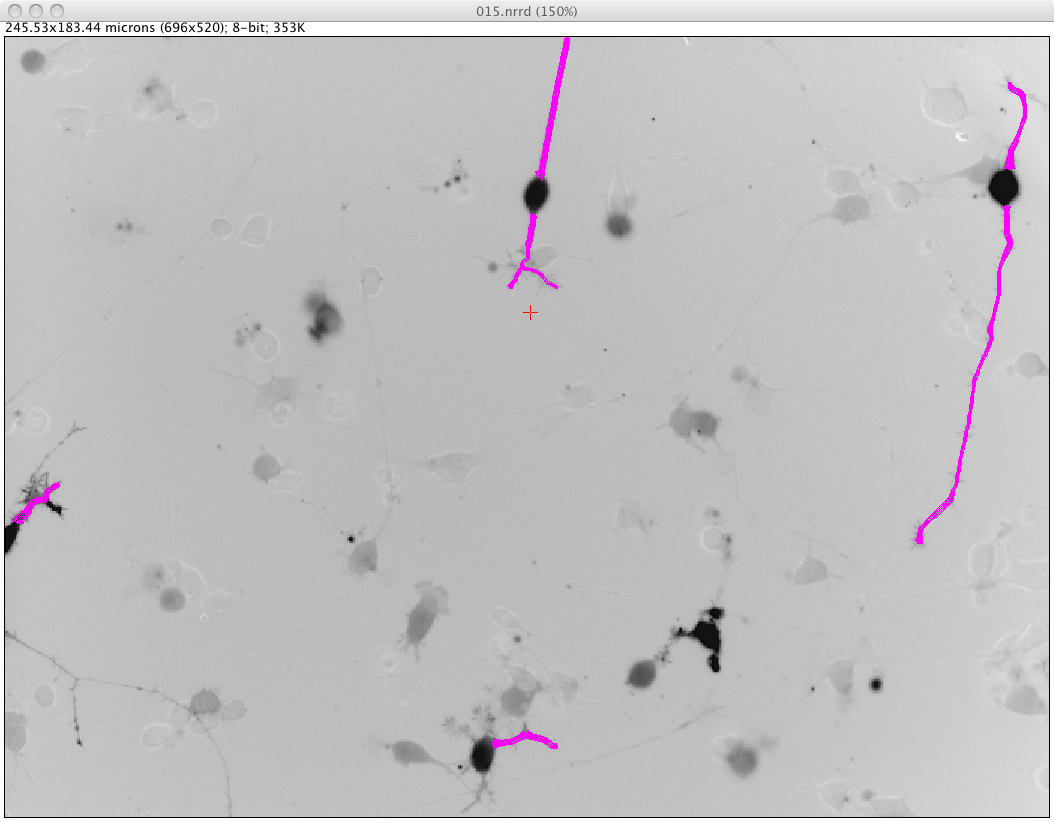
\includegraphics[width = 0.5\textwidth] {images/SNT_015_Seg.png}\\ 
%       \end{tabular} 
%    \caption{ \footnotesize  Ground truth annotation. First row, neuron tracking annotation using the \texttt{TrakEM2} plugin. Two different time frames are displayed. 
%    Second row, Neurite trees annotation using the Simple Neurite Tracer plugin. On the left, the original image, and on the right the manual annotation overlaid on the image.}
%    \label{fig:annotations}
%  \end{center}
%\end{figure}
%%----------------------------------------------------------------------------


%======================================================
\subsection{Evaluating Cell body tracking}
%======================================================

%======================================================
\subsection{Evaluating Neurites detection}
%======================================================

%======================================================
\subsection{Evaluating Neurites association}
%======================================================

%======================================================
\section{Data structure }
%======================================================
TODO

%======================================================================
%\bibliographystyle{naturemag}
\bibliography{vision}
%======================================================================

%\begin{addendum}
% \item Put acknowledgements here.
% \item[Competing Interests] The authors declare that they have no
%competing financial interests.
% \item[Correspondence] Phone: +41 61 267 22 03; Fax: +41 61 267 35 66; E-mail : \texttt{olivier.pertz@unibas.ch}.
%\end{addendum}

\end{document}


















%======================================================================

%% Example Figure commented
%FFFFFFFFFFFFFFFFFFFFFFFFFFFFFFFFFFFFFFFFFFFFFFFFFFFFFFFFFFFFFFFFFFFFFF
%\begin{figure}
%\caption{Each figure legend should begin with a brief title for
%the whole figure and continue with a short description of each
%panel and the symbols used. For contributions with methods
%sections, legends should not contain any details of methods, or
%exceed 100 words (fewer than 500 words in total for the whole
%paper). In contributions without methods sections, legends should
%be fewer than 300 words (800 words or fewer in total for the whole
%paper).}
%\end{figure}
%FFFFFFFFFFFFFFFFFFFFFFFFFFFFFFFFFFFFFFFFFFFFFFFFFFFFFFFFFFFFFFFFFFFFFF

%Figures
%Figure 1. Global pipeline to analyze neurite outgrowth morphodynamic phenotypes. (olivier and Ludo)
%Figure 2. Computer vision segmentation of neuronal morphodynamics feature extraction.
%(Fethallah and Kevin)
%Figure 3.  Description of morphodynamic features.
%(Fethallah and Kevin)
%Figure 4. Morphodynamic phenotype feature selection
%(Riwal)
%try to make a  series of schemes that explain the different steps in feature selection,
%vector distance, assessment of interplate and siRNA induced noise.
%
%Figure 5.  Morphodynamic phenotype description.
%(Riwal, Olivier, Ludo)
% this will consist of a color-coded map of the different features extracted for each gene perturbation, we will then focus on more specific aspects of what we learned.
%
% 
%Supplementary Figures.
%
%Figure S1. Experimental controls lifeact-GFP/NLS-mCherry reporter and siRNA transfection.
%(a) Structure of the Lifeact-GFP IRES NLS-mCherry expression vector. (b) Effect of Lifeact-GFP expression on neurite outgrowth.
%(ludo and olivier)
%
%
%Figure S2. Feature selection on synthetic data produced by mixing videos from different known sources to test the ability of the algorithm to appropriately identify different morphodynamic signatures (Riwal)
%
%
%
%?
%
%Supplementary tables.
%
%Table S1. Definition of static features.
%Table S2. Definition of dynamic features.
%
%
%
%?
%Supplementary notes
%
%Supplementary note 1. Description of RNA interference experiments.
%
%Olivier and ludo
%
%Supplementary note 2. Description of microscope setup used for high content acquisition.
%Olivier and ludo
%
%
%Supplementary note 3. In depth description of computer vision segmentation and evaluation of the method by comparison with ground truth.
%
%Fethallah and Kevin
%
%
%Supplementary note 4. Description of html format in which the cell trajectories are described
%
%Fethallah and Kevin
%
%?
%Supplementary movies.
%
%Supplementary movie 1. Representative timelapse movie of N1E-115 cells expressing the GFP-lifeact-IRES-NLS-mcherry construct with the 10x PlanApo objective.
%
%Supplementary movie 2. Representative timelapse movie of N1E-115 cells expressing the GFP-lifeact-IRES-NLS-mcherry construct with the 20x PlanApo objective.
%
%Supplementary movie 3.
%
%
%
%
%
% 
%References
%
%1.	B. Snijder, R. Sacher, P. Ramo et al., Nature 461 (7263), 520 (2009).
%2.	C. Collinet, M. Stoter, C. R. Bradshaw et al., Nature 464 (7286), 243 (2010).
%3.	M. Held, M. H. Schmitz, B. Fischer et al., Nature methods 7 (9), 747 (2010).
%4.	D. Loerke, Q. le Duc, I. Blonk et al., Science signaling 5 (231), rs5 (2012).
%5.	J. Riedl, A. H. Crevenna, K. Kessenbrock et al., Nature methods 5 (7), 605 (2008).

